\documentclass{article}
\usepackage{fullpage}
\usepackage{amsmath}
\usepackage{url}
\usepackage{verbatim}
\usepackage{graphicx}
\DeclareGraphicsExtensions{.pdf,.png,.jpg}
\usepackage[square, comma, sort&compress]{natbib}
\usepackage{wrapfig}
\usepackage{float}
\usepackage{color}
\usepackage[section]{placeins}

\DeclareMathOperator*{\E}{\mbox{\large E}}

\newcommand{\approptoinn}[2]{\mathrel{\vcenter{
  \offinterlineskip\halign{\hfil$##$\cr
    #1\propto\cr\noalign{\kern2pt}#1\sim\cr\noalign{\kern-2pt}}}}}

\newcommand{\appropto}{\mathpalette\approptoinn\relax}

\def\app#1#2{%
  \mathrel{%
    \setbox0=\hbox{$#1\sim$}%
    \setbox2=\hbox{%
      \rlap{\hbox{$#1\propto$}}%
      \lower1.1\ht0\box0%
    }%
    \raise0.25\ht2\box2%
  }%
}
\def\approxprop{\mathpalette\app\relax}

\begin{document}
\large

\title{Haplotype-based variant detection from short-read sequencing}
%\title{Characterization of complex variants by haplotype-based variant detection}

\author{Erik Garrison and Gabor Marth}

\maketitle


\begin{abstract}

With genomic variant detection methods, we can determine point-wise differences against a reference genome.  Widely-used methods fail to reliably characterize the relative phase of proximal alleles.  This information is essential for the functional interpretation of genomic material, and can be determined directly from the primary sequence reads.  Here we propose such a method, and demonstrate that the use of haplotypes does not only improve our ability to interpret genomic information, and affords a large improvement in detection performance over existing methods.  We implement our approach in the \emph{freebayes} Bayesian variant detector.  To do so, we extend the now-ubiquitous Bayesian variant detection model to allow for arbitrary genome architecture, ploidy, population structure, numbers of samples, and numbers of alleles.  To further improve performance, we extend the model to incorporate an estimate of our confidence that the locus and alleles under analysis can be characterized accurately using our experimental data.  These advances allow \emph{freebayes} to outperform all existing variant detection methods at the detection of SNPs, indels, and small complex variants.


\end{abstract}



\section{Motivation}

\begin{comment}
write introduction / motivation statement to lead into results

\emph{
GTM: Biological motivations: 
(1) Haplotype phasing: [Result: resolution of compound hets. e.g. BLM allele-like situations such as the frame-restoring indels, and the 6 SNPs in a row. This improves functional impact prediction] [Display items: example of phase-restoring INDELs]
(2) Complex variant detection: [Result: Alleles are reported in a consistent fashion, allowing e.g. improved genotyping chip design] [Display items: OMNI results]
(3) Accuracy of SNP and INDEL detection improves because haplotype-level detection improves signal to noise ratio [Result: comparison to other SNP calls and INDEL calls; 1bp INDEL detection accuracy as a function of clump size] [Display items: SNP AUC table; INDEL size as a function of clump size; INDEL caller ROC comparison]
(4) Enables integration of multiple independent callsets. [Results: comparison to other integration strategies; Quoting number of inconsistent allele locations in Phase 1.] [Display items: cartoon of inconsistent calls; table comparing performance of variant consolidation methods]
(5) Ploidy framework allows accurate genotype determination in haploid regions. [Result: Chromosome X calling]. [Display items: in-text chromosome X results]
(6) Physical haplotype method gives better sensitivity than assembly based methods (local or global), but comparable to mapping methods, while achieving better specificity.  [Results: SNP AFS comparison across mapping, assembly methods] [Display items: AFS comparison; call comparison table]
}

\emph{
Gabor's logical ordering: 1, 2, 4, 3, 6, 5
}

\emph{
Literature/competing method review:
How other methods deal with the same issues?
Other approaches for variant calling (per-site mapping based, assembly, local assembly)
How our approach promises to solve the problems.
}

\end{comment}


While \emph{statistical phasing} approaches are necessary for the determination of large-scale haplotype structure \citep{browning2007, mach2010, delaneau2012, howie2011}, sequencing traces provide short-range phasing information that may be employed directly in primary variant detection to establish phase between proximal alleles.  Present read lengths and error rates limit this \emph{physical phasing} approach to variants clustered within tens to hundreds of bases, but as the cost of obtaining long sequencing traces decreases \citep{branton2008, clarke2009}, physical phasing methods will enable the determination of larger haplotype structure directly using only sequence information from a single sample.

Haplotype-based variant detection methods, in which short haplotypes are read directly from sequencing traces, offer a number of benefits over methods which operate on a single position at a time. Haplotype-based methods ensure semantic consistency among described variants by simultaneously evaluating all classes of alleles in the same context. 
Locally phased genotypes can be used to improve genotyping accuracy in the context of rare variations that can be difficult to impute due to sparse linkage information.

Similarly, they can assist in the design of genotyping
assays, which can fail in the context of undescribed variation at the assayed locus.  These methods can provide the direct detection of complex variants of clinical significance, such as the BLM\textsuperscript{Ash} allele, a complex block substitution in a helicase gene related to cancer risk \citep{blmash} or recurrent multi-nucleotide polymorphisms often found in particular cancer types \citep{recurrentTERT2013}.  Directly detecting such alleles from sequencing data decreases the cost of secondary, manual analysis of detected variants, a significant diagnostic cost now generally accepted as necessary for the accurate reporting of non-SNP variation in clinical diagnostic contexts.

The use of longer haplotypes in variant detection can improve detection by increasing the signal to noise ratio of the genotype likelihood space that is used in analysis, provided some degree of independence between sequencing errors.  This follows from the fact that the space of possible erroneous haplotypes expands dramatically with haplotype length, while the space of true variation remains constant, with the number of true alleles less than or equal to the ploidy of the sample at a given locus.

The direct detection of haplotypes from alignment data presents several challenges to existing variant detection methods.  As the length of a haplotype increases, so does the number of possible alleles within the haplotype, and thus methods designed to detect genetic variation over haplotypes in a unified context must be able to model multiallelism.  However, most variant detection methods establish estimates of the likelihood of polymorphism at a given loci using statistical models which assume biallelism \citep{li2011stats,marth99} and uniform, typically diploid, copy number \citep{gatk2011}.  Moreover, improper modeling of copy number impedes the accurate detection of small variants on sex chromosomes, in polyploid organisms, or in locations with known copy-number variations, where called alleles, genotypes, and likelihoods should reflect local copy number and global ploidy.

To enable the application of population-level inference methods to the detection of haplotypes, we generalize the Bayesian statistical method described by \citet{marth99} to allow multiallelic loci and non-uniform copy number across the samples under consideration.  We have implemented this model in FreeBayes \citep{freebayesgit}.  In addition to extensions enabling haplotype-based detection, we have incorporated a model of the capacity for the alignments to characterize the locus and alleles in question into our prior probability.


\section{Results}

\subsection{Small variant detection in simulated data}
\label{sec:simulation}

%\emph{GTM: This section presents results for Biological problem 3. The table for SNPs, and the figure for INDELs.}

To assess the performance of our method, we used the population genome simulator mutatrix \citep{mutatrixgit} to simulate variation in 100 samples over 100 kilobases of human chromosome 20, and the mason read simulator \citep{holtgrewe2010} to generate a simulated Illumina-like 70bp-reads at 10x depth per sample.
%several sets of simulated data: 10 samples at 100x coverage, 1000 samples at 10x coverage, and a single sample at 20x, 50x, 100x, and 200x coverage, over 100 kilobases of human chromosome 20.
%This simulator employs a $1/i$ allele frequency model to simulate SNPs and indels across a number of samples.
The data were aligned with Mosaik \citep{mosaik}, and variants were called using several popular detection methods capable of simultaneously detecting SNPs and short indels: GATK HaplotypeCaller and UnifiedGenotyper (version 2.7.4) \citep{gatk2011}, samtools (version 0.1.19-44428cd) \citep{samtools}, and FreeBayes (version 0.9.9.2-21-g78714b8).
%In order to improve statistical power, each simulation was run 100 times and the results were merged.
To assess each caller's detection performance we generated receiver-operator characteristics (ROCs) using vcfroc \citep{vcflibgit}.  We provide results in terms of area under the curve (AUC) for all tested variant callers in table \ref{tab:simROCs}.%  (See supplement for ROC plots for each simulation.)

These results indicate that FreeBayes provides superior performance to the GATK and samtools at all assayed depths and numbers of samples.
%For both SNPs and indels, the relative performance difference between FreeBayes and these other methods is largest at low sequencing depth and numbers of samples, and diminishes as sequencing depth or number of samples increases.
We observe that the difference in the AUC metric is dominated by both minimum distance from perfect discrimination (perfect sensitivity and perfect specificity), in which FreeBayes consistently outperforms the other methods, and by apparent hard limitation on sensitivity imposed by the other methods.  We hypothesize that the difference in performance for indels, which is larger than that for SNPs, reflects our method's detection of alleles on haplotypes, which improves the signal to noise ratio of the and effectively removes low-frequency alignment artifacts without the need for out-of-band indel and base-quality recalibration methods (we further explore this in \ref{sec:indelerror}).



\begin{figure}[h!]
\centering
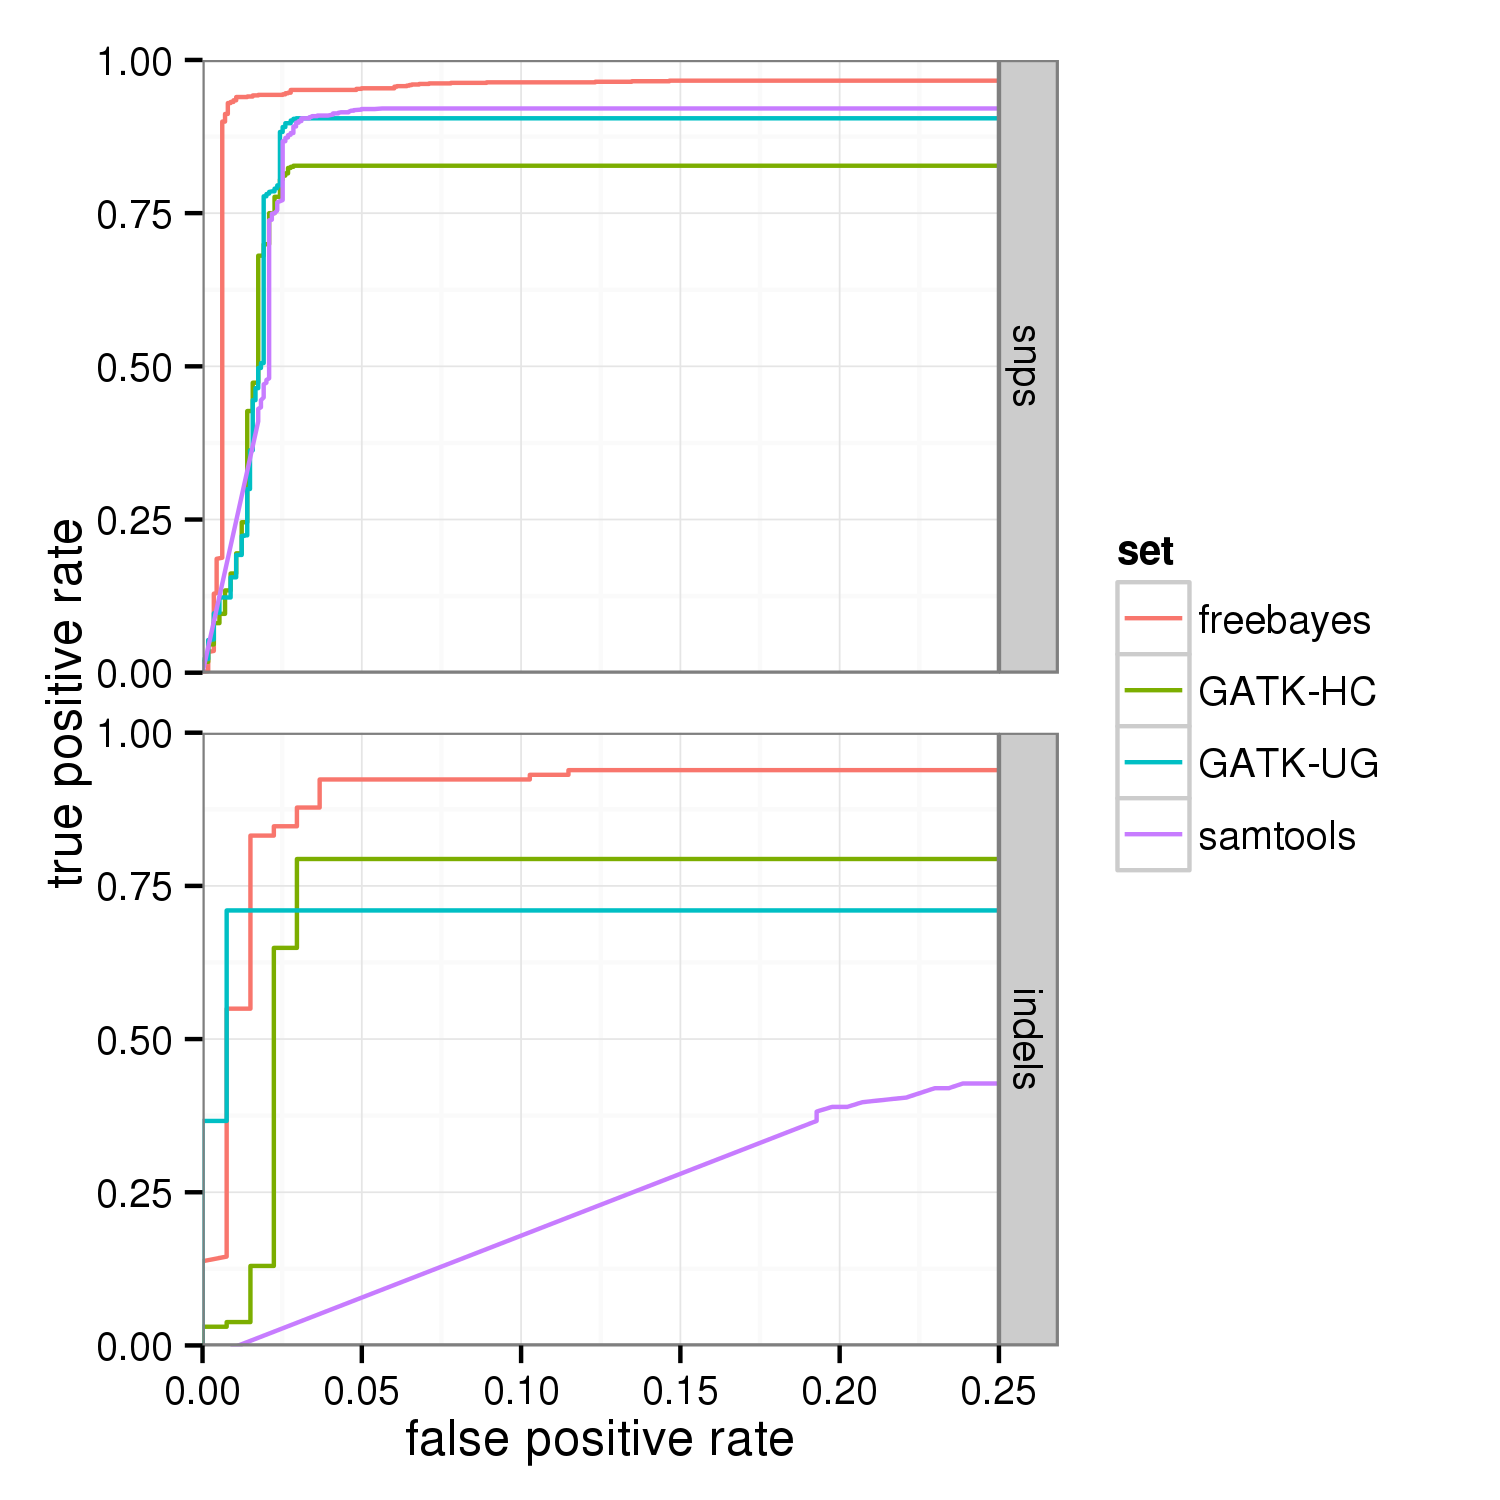
\includegraphics[width=0.7\textwidth]{100samples10x_0_25_both}
\caption{Receiver-operator characteristics (ROCs) for FreeBayes, GATK HaplotypeCaller and UnifiedGenotyper, and samtools on 100 samples at 10x simulated sequencing depth.  FreeBayes achieves the highest area under the curve (AUC) \ref{tab:simROCs}, with the HaplotypeCaller and samtools each performing next-best for indels and SNPs, respectively.}
\label{fig:10xROC}
\end{figure}


\begin{table}
\centering
    \begin{tabular}{|l||l|l|l|l|}
        \hline
        variant detector      & depth            & samples  & AUC SNPs                & AUC indels                \\ \hline
        FreeBayes             & 10               & 100      & 0.9594                  & 0.9400                 \\ 
        \hline
        GATK HaplotypeCaller  & 10               & 100      & 0.8155                  & 0.7765                 \\ 
        \hline
        GATK UnifiedGenotyper & 10               & 100      & 0.8907                  & 0.7073                 \\ 
        \hline
        samtools              & 10               & 100      & 0.9056                  & 0.4698                 \\  \hline
    \end{tabular}

\caption{Performance of FreeBayes, GATK HaplotypeCaller and UnifiedGenotyper, and samtools against simulated data.
%FreeBayes provides the best area under the curve (AUC) at all sequencing depths and numbers of samples for both SNPs and indels.}
}
\label{tab:simROCs}
\end{table}


\subsection{Using simulation to assess the direct detection of haplotypes}
\label{sec:complexsimulation}

In order to facilitate our assessment of the method at determining phase between clusters of alleles, we set a mutation rate sufficient to generate many clusters of variants in these simulated samples.  We then simulated reads at 20x coverage from the resulting simulated chromosomes using wgsim \citep{samtools}, aligned the results using Mosaik \citep{mosaik} and ran freebayes on the resulting alignments specifying a haplotype detection length of 10bp.  The results were compared to the truth set produced by mutatrix using the utility vcfgeno2haplo in vcflib \citep{vcflibgit} which can construct haplotype observations of a given length from phased genotype information like that produced by mutatrix.
%For the evaluation of complex alleles detection, we ignored haplotypes which could not be detected by the algorithm given the maximum haplotype length constraint of the detection method.

Our results agree with those obtained for other classes of small variants in section \ref{sec:simulation}, showing high performance against SNPs (AUC of 0.979) and indels (AUC of 0.948).  For complex variants composed between multiple small variants, direct detection provides an AUC of 0.919.

% TODO rerun using newest freebayes version

% humu.bc.edu:haplotypecomparisons/1mb_10x_10samples
%> abs(trapz(c(1, roc$snpsfpr), c(1, roc$snpstpr)))
%[1] 0.9795195
%> abs(trapz(c(1, roc$complexfpr), c(1, roc$complextpr)))
%[1] 0.9033818
%> abs(trapz(c(1, roc$indelsfpr), c(1, roc$indelstpr)))
%[1] 0.7524788
%> abs(trapz(c(1, roc$mnpsfpr), c(1, roc$mnpstpr)))
%[1] 0.9480347


%\section{Comparison of haplotype-based calls to statistically phased genotypes}


\begin{figure}[h!]
\centering
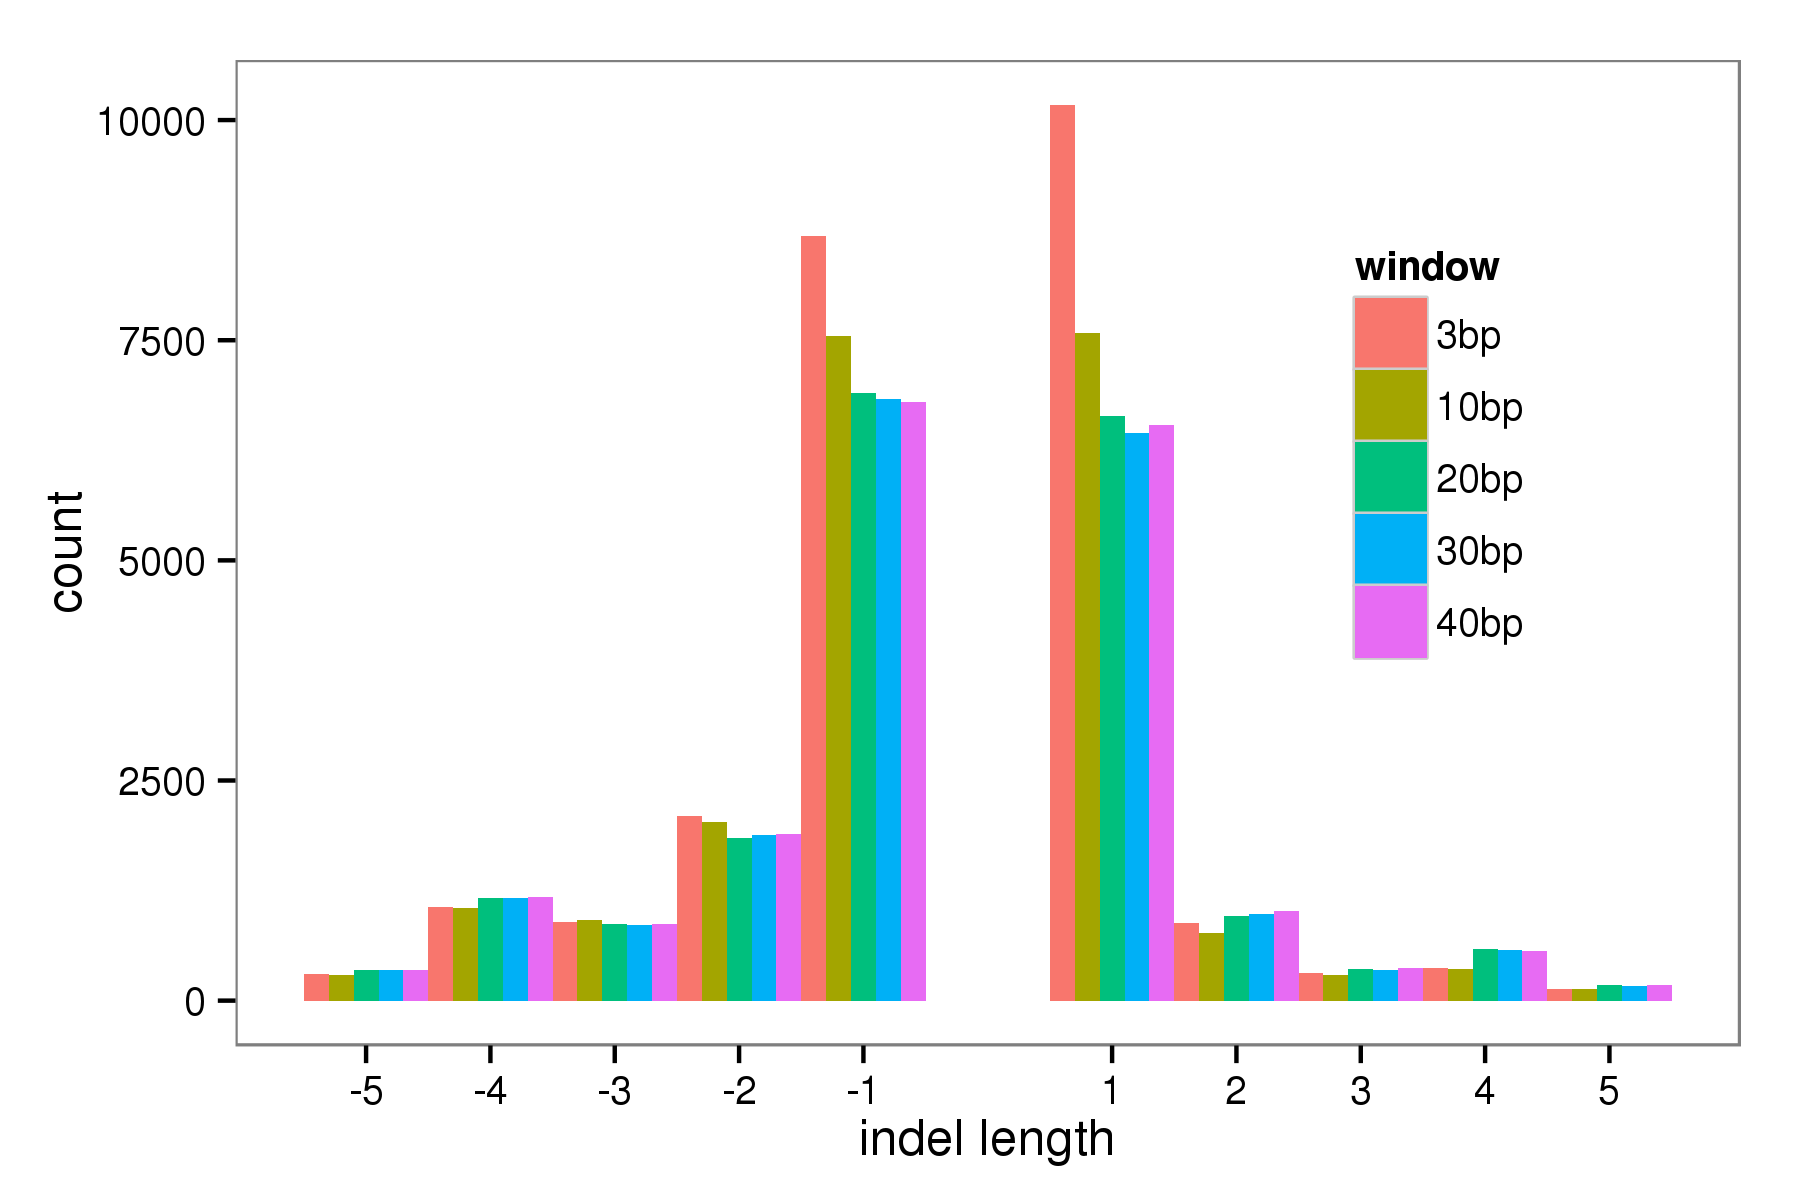
\includegraphics[width=0.8\textwidth]{indel_error}
\caption{A known error mode of Illumina sequencing methods generates a 1bp insertion artifact that is detected by standard mapping-based variant calling methods.  The artifact results in a relative over-abundance of 1bp insertions.  Here, we characterize the ability of our method to remove this artifact by detecting variants in a larger detection window.  As the calling window size is increased beyond 10bp, the artifact is effectively removed, and the balance between insertions and deletions at a given length normalizes.}
\label{fig:indelerror}
\end{figure}


\subsection{Using haplotype-based variant detection to improve the signal to noise ratio of candidate variants}
\label{sec:indelerror}

The fluorescence-based imaging utilized by Illumina sequencing machines is susceptible to errors generated by air bubbles introduced into the flowcell in which the sequencing reaction takes place.  Bubble errors tend to manifest themselves as high-quality 1bp insertions in sequencing traces derived from spots in the affected regions of the sequencing flowcell.  These errors are randomly distributed with respect to reference position, but their high frequency in some sequencing runs means that they will spuriously be detected by single-position mapping-based variant detectors when they overlap positionally.  We can observe the presence of this error because it causes a preponderance of 1bp insertions over deletions.  Typically, 1bp insertions are discoverable in human genomes at a slightly lower frequency than deletions, and thus this error process can be observed by inspection of the indel length-frequency distribution.

To assess the ability of our haplotype-based method to overcome this characteristic error, we detected variants in the previously described AFR191 sample set using a number of different haplotype lengths.  The indel detection results (figure \ref{fig:indelerror}) indicate that this error mode can be effectively removed from small variant calls by increasing the detection window size to 10bp or greater.

As we increase the length of detected haplotypes, we increase the number of possible erroneous haplotypes without increasing the number of true haplotypes.  This effect results in an improved signal to noise ratio for detected variants at larger haplotype sizes.  As such, increasing window size in our algorithm allows us to exclude likely insertion artifacts from consideration, as the recurrance of an erroneous haplotype diminishes rapidly with haplotype length.  We hypothesize that this effect dominates the improvement in specificity yielded by assembly methods.  However, if window sizes are fixed, as is the case in the existing implementations of such methods, sensitivity to rare variation will suffer (discussed in section \ref{sec:lowfreq}).


%\begin{wrapfigure}{r}{0.3\textwidth}
%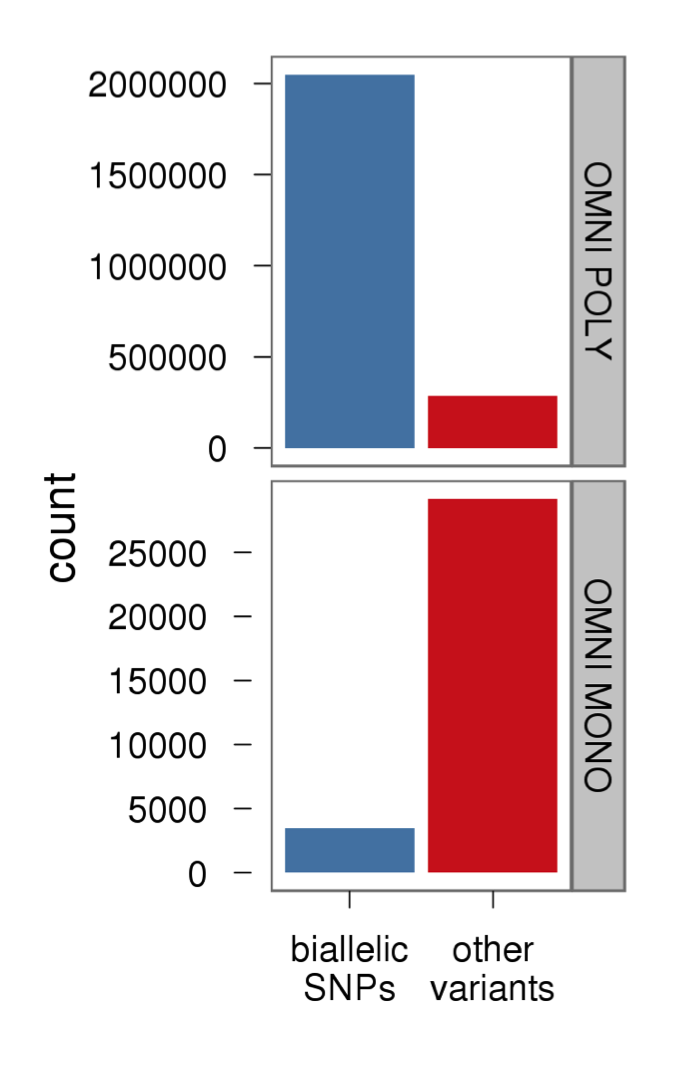
\includegraphics[width=0.3\textwidth]{omni_errors}
%\caption{Omni errors.}
%\label{fig:omnierrors}
%\end{wrapfigure}

\begin{figure}[h!]
\centering
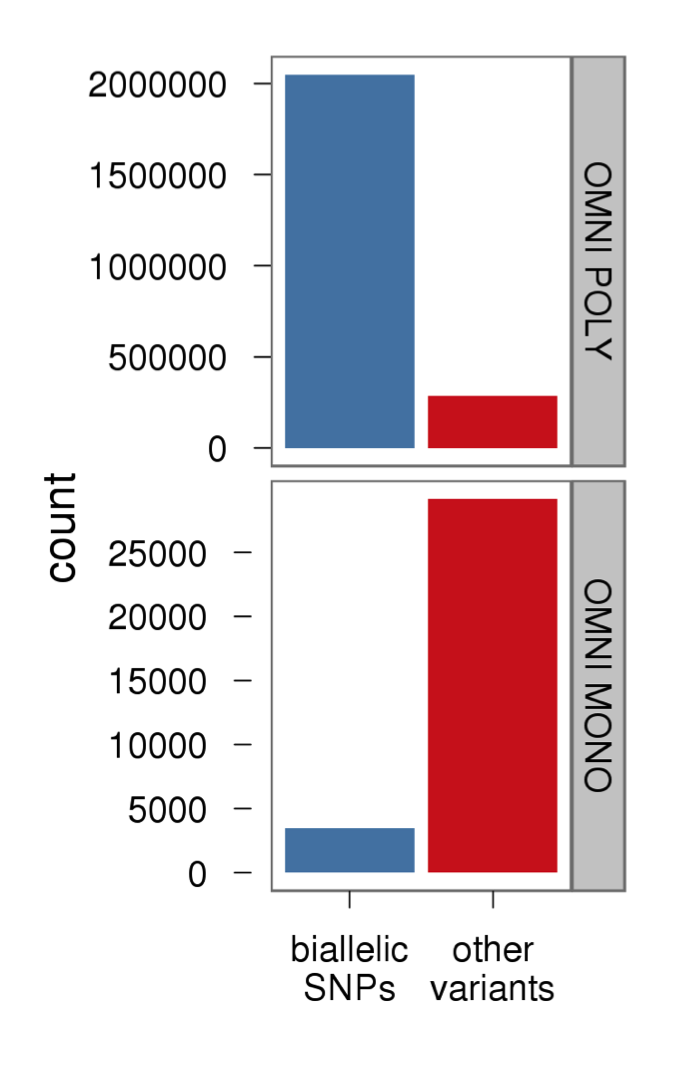
\includegraphics[width=0.3\textwidth]{omni_errors}
\caption{The Omni 2.5 genotyping array includes a number of alleles which consistently report as non-polymorphic (monomorphic) in the 1000 Genomes cohort in which they were originally detected.  By detecting variants using our method at a 10bp variant calling window, we demonstrate that more than 90\% of the apparently monomorphic loci are not biallelic SNPs, and thus the array design does not match the local variant structure in these samples.  By using a haplotype-based approach, groups designing genotyping arrays can avoid this common error mode.}
\label{fig:omnierrors}
\end{figure}


\subsection{Using haplotype-based variant detection to understand genotyping array design failure}
\label{sec:arrayfailure}

Variant calls generated during the pilot phase of the 1000 Genomes Project \citep{1000Gphase1} were used to design a genotyping array, (the Illumina OMNI2.5).  Subsequently, many of the alleles on this array (approximately 10\%) were found to be putatively monomorphic in the same set of samples, suggesting they resulted from variant detection error.

We investigated these loci using whole-genome calls in the low-coverage cohort in Phase I of the 1000 Genomes Project.  We ran freebayes using a haplotype window of 10 base pairs.  On comparison with the monomorphic array loci, we found that approximately 90\% of the array-monomorphic loci overlap non-SNP or non-biallelic variation in these samples within 10bp of the target SNP, whereas the opposite is true of polymorphic loci--- greater than 90\% of loci assayed as polymorphic overlap biallelic SNPs.

We observe that many of the apparent failures in variant detection are actually caused by an inability of methods to assess local clusters of variation.  The accurate design of genotyping arrays and their use in cross-validation of sequencing-based genotyping performance thus requires information about local haplotypes structure.

\subsection{The importance of accurately modeling copy number variations on sex chromosomes}

Our method is currently the only variant detector in common use which provides the ability to call males and females jointly on chromosome X with correct copy number.  To evaluate the benefits of this approach, we detected variants in chromosome X for 191 low-coverage 1000 Genomes samples of African ancestry using FreeBayes both with and without copy-number awareness.  Comparison of our results to the genotyping array calls (excluding cases of likely array failure due to non-SNP, non-biallelic variation as described in section \ref{sec:arrayfailure}) indicates that when calling without copy-number awareness, our genotyping error rate was 7.28\%, whereas when calling with awareness of copy-number, the genotyping error rate is only 3.55\%.  The relatively high error rate is typical in the case of low-coverage data.  The difference in overall error rate suggests that there is substantial benefit to directly modeling copy number within the variant detection process.


\subsection{Comparing to other methods in low-coverage sequencing data}
\label{sec:1000Gcomparisons}

In the testing phase of the 1000 Genomes Project, participating groups submitted callsets based on 191 samples of African ancestry (AFR191).  Results are characterized in figure \ref{table:1000Gcomparisons}.  Unlike other haplotype-based and assembly metods, the approach described in this paper (BC2) provides sensitivity to known variants equivalent to mapping-based methods (BCM, BC1, SI1, UM).  Furthermore, the method's ability to characterize haplotypes in loci which appeared to be monomorphic on the Omni genotyping array allows for discrimination against known artifacts as good as the best mapping-based detection pipelines.  Thus we achive a result which is nearly equivalent in sensitivity to the most-sensitive mapping-based method (BCM) and of a similar specificity to that achieved by assembly methods (OX2, SI2 BI2).

\begin{table}
\resizebox{\textwidth}{!}{%
\centering
\begin{tabular}{|l|lllll|lll|ll|lllll|}
\hline
call set       & BC   & BCM  & BI1  & SI1  & UM   & BC2  & BI2  & OX1  & SI2  & OX2  & Union  & 2/9  & 3/9  & 4/9  & BC cons   \\
\hline
SNPs [K]       & 459  & 512  & 481  & 480  & 491  & 495  & 362  & 452  & 252  & 101  & 621  & 548  & 518  & 487  & 543       \\
Omni poly [\%] & 91.6 & 98.9 & 96.5 & 95.2 & 97.6 & 97.4 & 88.4 & 87   & 83.1 & 44.6 & 99.3 & 98.9 & 98.6 & 97.6 & 98.7 \\
Hapmap [\%]    & 94.5 & 99.4 & 98   & 95.6 & 98.9 & 98.3 & 93.6 & 90.3 & 91.1 & 53.7 & 99.4 & 99.4 & 99.3 & 99   & 98.6 \\
Omni mono [\%] & 1.39 & 1.63 & 0.29 & 0.62 & 0.77 & 0.56 & 0.14 & 1.1  & 0.72 & 0.1  & 3.73 & 0.97 & 0.67 & 0.48 & 0.65 \\
\hline

\hline
\end{tabular}}
\caption{Performance of various variant detection pipelines tested as part of the 1000 Genomes Project.  Sets are Boston College; non-haplotype-based method (BC), haplotype-based method described in this paper (BC2), Baylor College of Medicine (BCM), Broad Institute GATK UnifiedGenotyper (BI1), Sanger Institute Samtools (SI1), University of Michigan GlfMultiples (UM), Broad Institute GATK HaplotypeCaller (BI2), Oxford Platypus (OX1), Sanger SGA (SI2), Oxford Cortex (OX2).  Union: combination of all variants detected in component methods.  2/9, 3/9, 4/9: voting-based consensus results.  BC cons: haplotype-based ensemble method.}
\label{table:1000Gcomparisons}
\end{table}



%\begin{figure}[h!]
%\centering
%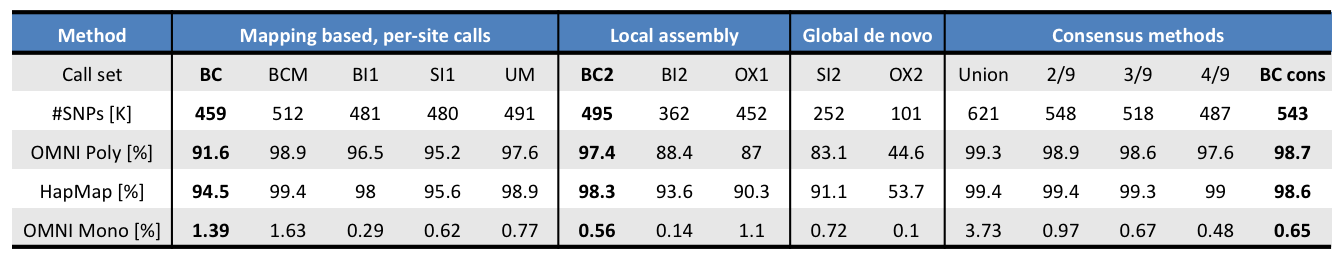
\includegraphics[width=1.0\textwidth]{1000G_performance_comparison}
%\end{figure}


\subsection{Indel detection performance}
\label{sec:1000Gindels}

\begin{table}
\centering
\begin{tabular}{|l||l|l|l|l|l|}
\hline
center           & specificity & sensitivity & caller & optimality &  AUC   \\
\hline
Oxford Cortex    & 98          & 27          & OX2    & 73.02739   & 0.2646 \\
Pindel           & 90          & 52          & Pindel & 49.03060   & 0.4680 \\
BC               & 83          & 66          & BC     & 38.01316   & 0.5478 \\
Broad assembly   & 80          & 67          & BI2    & 38.58756   & 0.5360 \\
Sanger           & 76          & 69          & SI1    & 39.20459   & 0.5244 \\
Broad mapping    & 65          & 74          & BI1    & 43.60046   & 0.4810 \\
Oxford Platypus  & 60          & 55          & OX1    & 60.20797   & 0.3300 \\ \hline
\end{tabular}
\end{table}


\begin{figure}[h!]
\centering
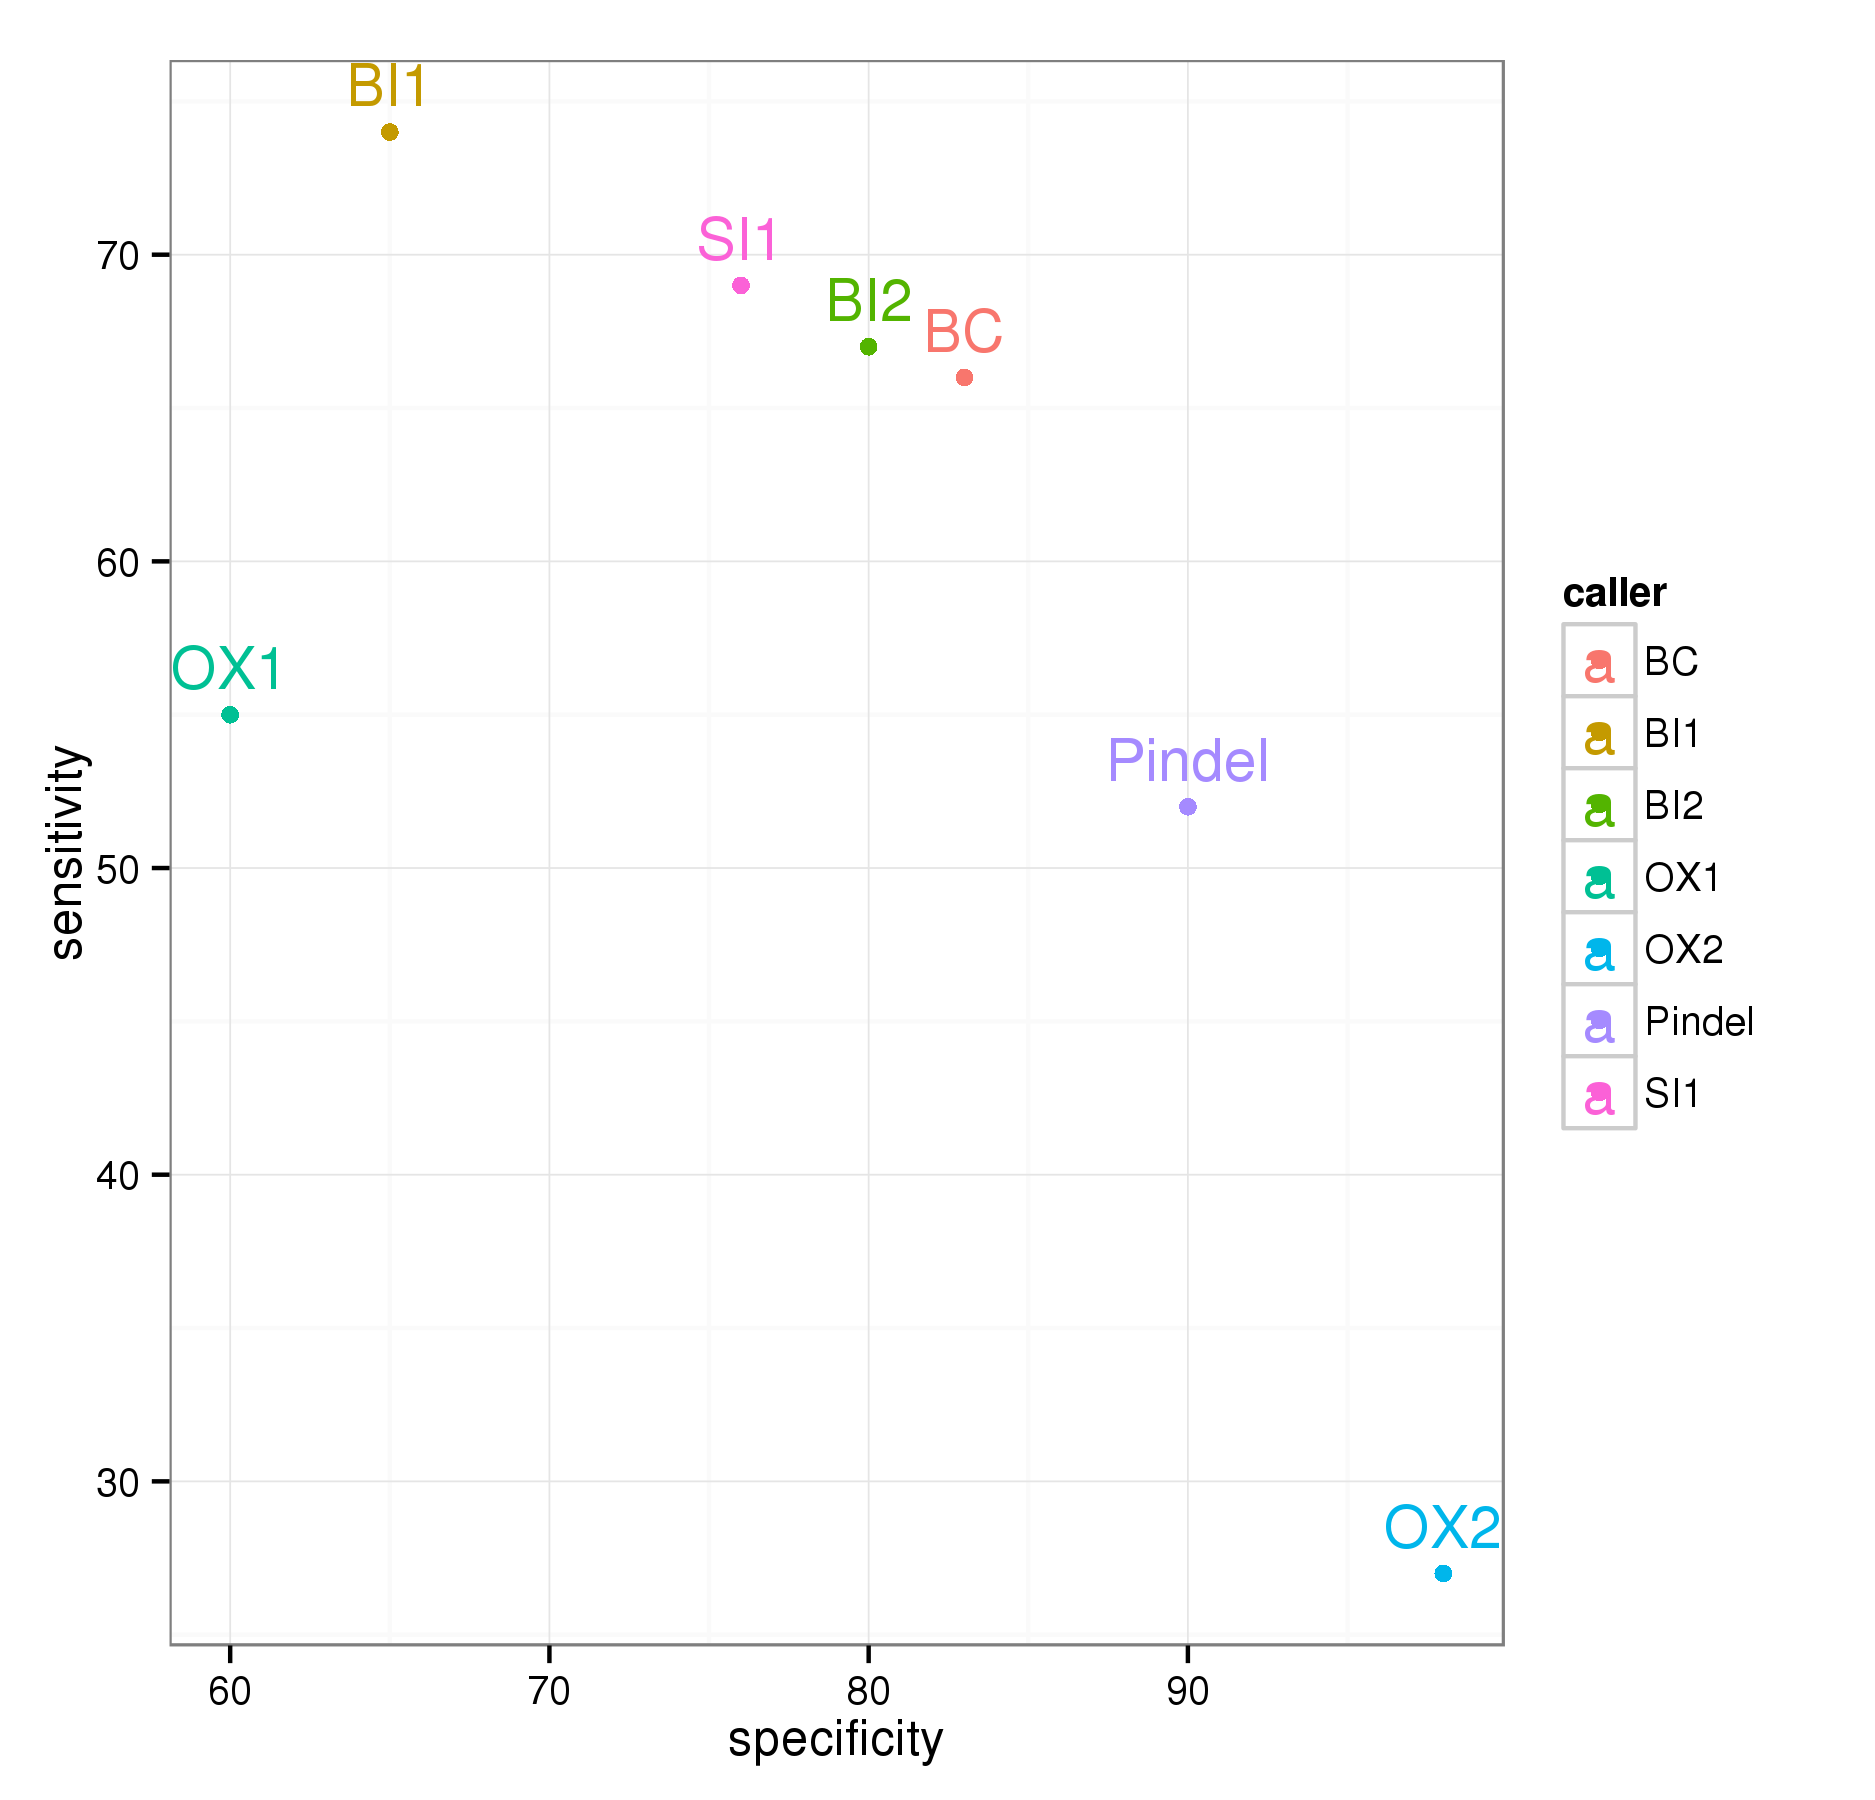
\includegraphics[width=0.6\textwidth]{miseq}
\caption{Performance of indel detection methods in 1000 Genomes project on the AFR191 sample set as assesed via high-depth resequencing validation.  Sets are Boston College FreeBayes (BC), Broad Institute GATK UnifiedGenotyper (BI1), Sanger Institute Samtools (SI1), Broad Institute GATK HaplotypeCaller (BI2), Oxford Platypus (OX1), Oxford Cortex (OX2).}
\label{fig:1000Gindels}
\end{figure}

\subsection{Sensitivity to low-frequency variation}
\label{sec:lowfreq}

Current methods for haplotype-based variant detection rely on assembly methods, which can be applied globally \citep{cortex} or locally \citep{dindel}.  These methods remove reference bias from the analysis of short-read sequencing data, but the generation of assemblies of large genomes requires pruning of low-frequency kmer observations.  While low-frequency kmers are often generated by sequencing error, in many cases they represent true variation, and thus this pruning reduces the sensitivity of existing assembly methods to true low-frequency variants.  In many contexts it is important to accurately and sensitively assess low-frequency variation, such as in experiments involving large numbers of samples, in the detection of sub-clonal mutations in cancer, and in pooled sequencing projects such as viral and metaganomic studies.  Our method does provide direct description of haplotypes, but because these haplotypes are generated only where multiple variations segregate an observed haplotype from the reference, it maintains sensitivity to low-frequency variants.

Results from the experiments described in \ref{sec:1000Gcomparisons} demonstrate that our method, while acting as a form of local assembly, does not incur the same sensitivity penalties seen in both local and global assembly methods.  We assess this using the count of minor alternate alleles as reported by each caller (figure \ref{fig:lowfreqsens}).  These results indicate that both global and local assembly methods suffer significant decrease in sensitivity to low-frequency variants, although the effect is less severe for local assembly.  In this test our method performs as well or better than the GATK UnifiedGenotyper, which is purely mapping-based, the GATK HaplotypeCaller, which uses local assembly, and the string graph assembler (SGA) which is a global, reference-free assembly approach.

\begin{figure}[h!]
\centering
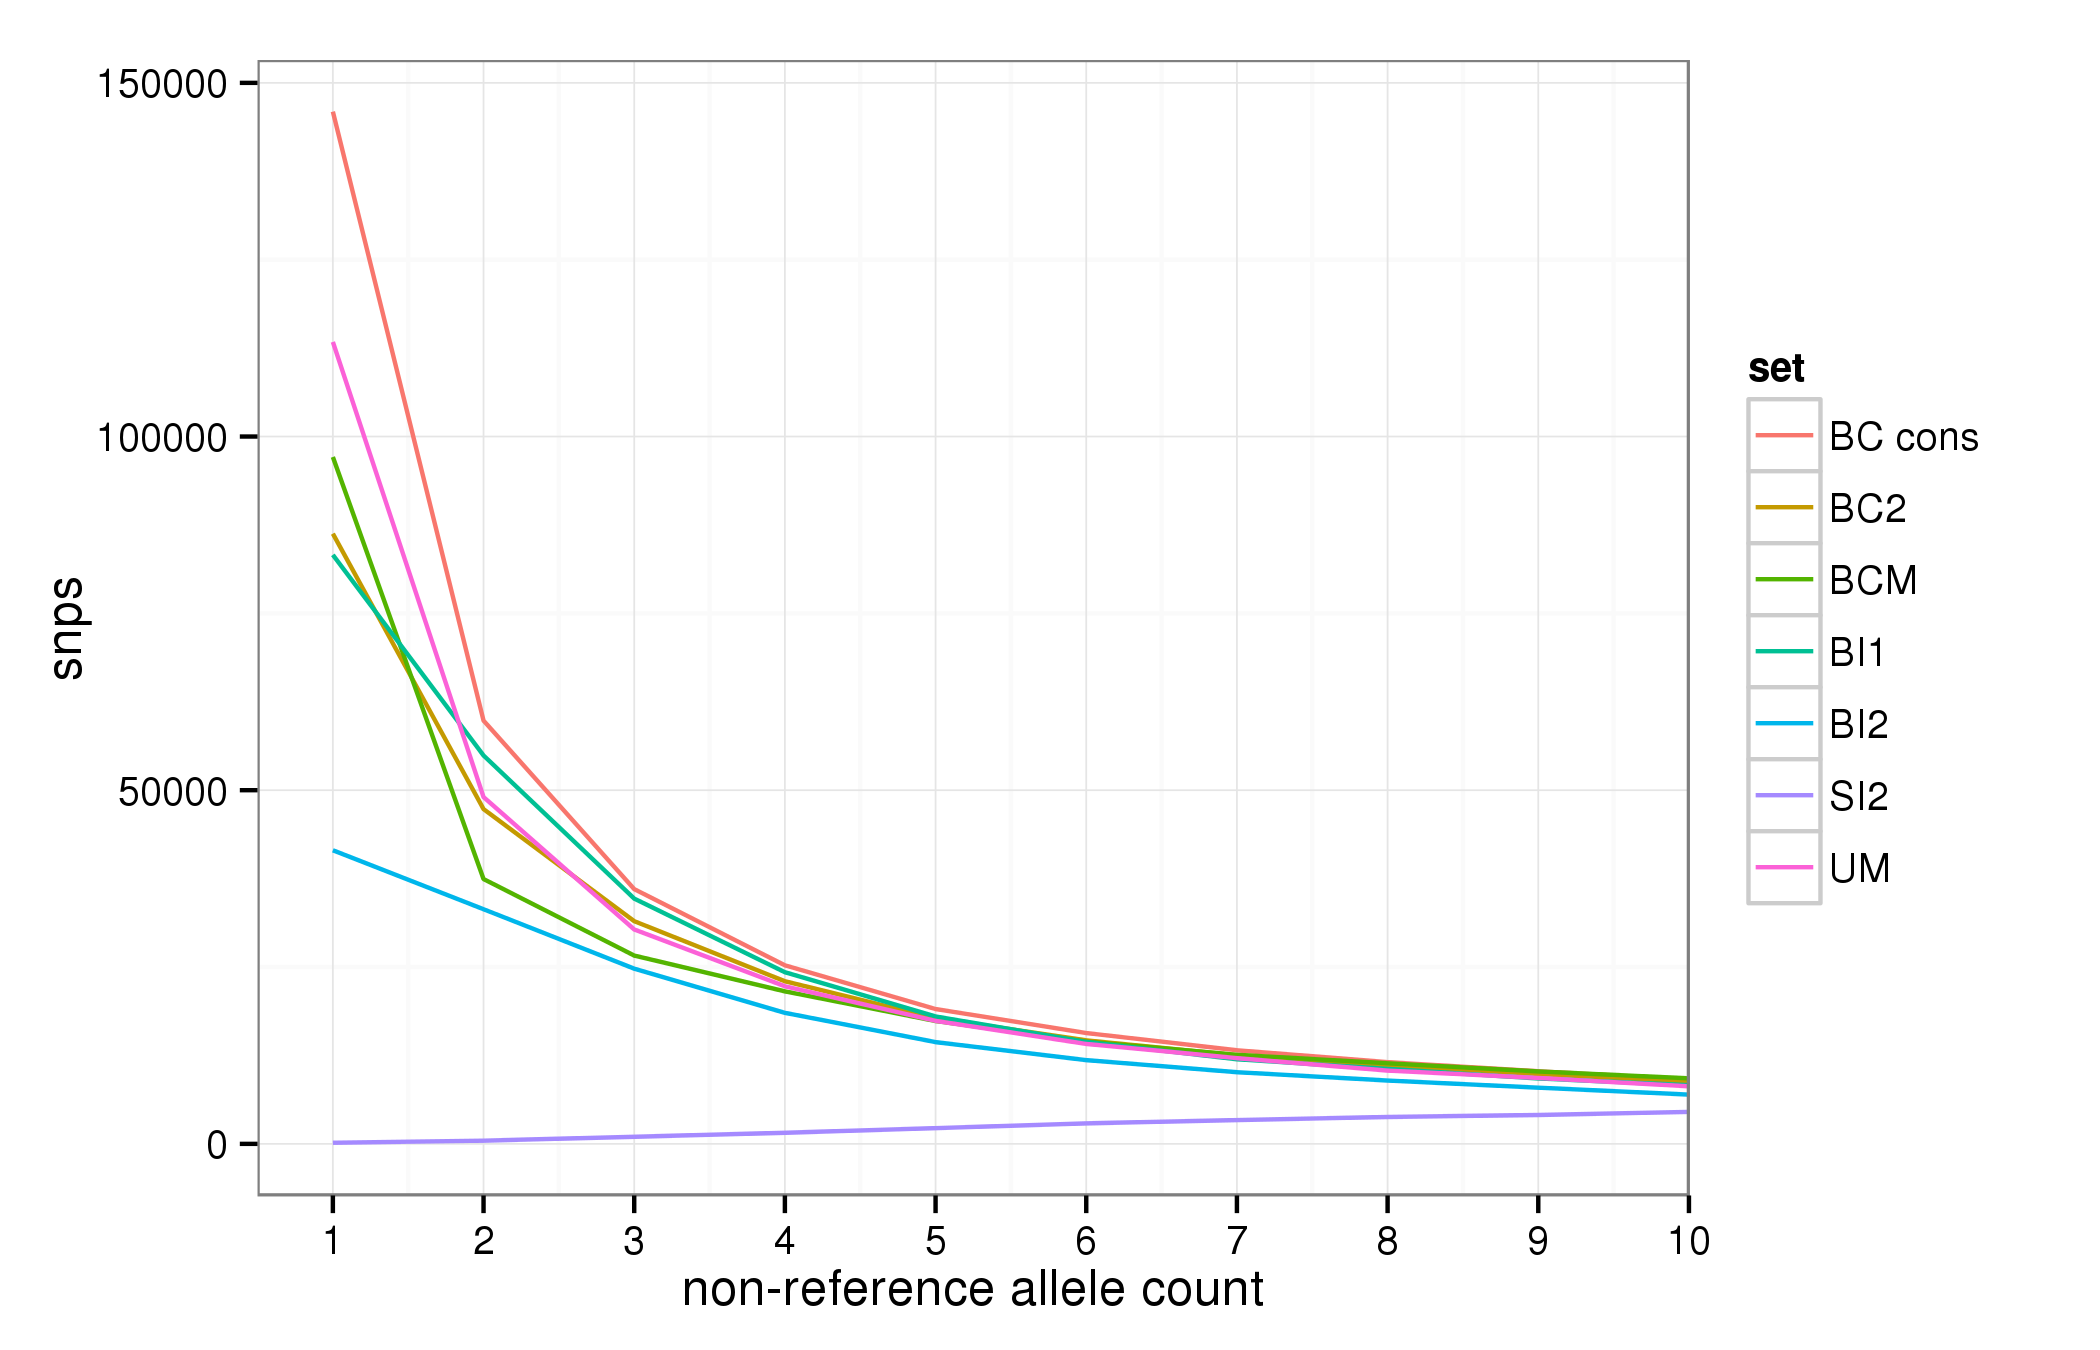
\includegraphics[width=0.8\textwidth]{low_frequency_sensitivity}
\caption{Sensitivity to low-frequency variants of various detection methods, as assessed in 191 samples of African ancestry in the 1000 Genomes low-coverage cohort.   BC2 is FreeBayes, BI1 is the GATK UnifiedGenotyper, BI2 is the GATK HaplotypeCaller, and SI2 is the global assembler SGA.}
\label{fig:lowfreqsens}
\end{figure}


\subsection{Haplotype-based consolidation of small variant calls}
\label{sec:ensemble}

Ensemble methods have been shown to provide superior performance to component inference methods in many contexts \citep{opmac99}.  We hypothesize that ensemble approaches to variant detection from short-read sequencing may provide improved performance in the context of variant detection.  While ensemble approaches have already been successfully applied to SNPs in large-scale resequencing projects \citep{1000GPhaseI}, their application to other variant classes is problematic because detectors can output the same allele in slightly different ways.  In the 1000 Genomes Phase I integrated callset, we find 181,567 cases in which incorrect description of small variants results in an ``impossible'' haplotype, such as where a small variant is phased inside of of a deletion, or multiple deletions overlap within 50 base pairs.  We can avoid such errors by using an approach that establishes the local haplotype structure around variants prior to using statistical phasing approaches to estimate large-scale haplotypes.



%\section{Generalizing variant detection to multiallelic loci and non-uniform copy number}
\section{Methods}
\label{sec:model}

\subsection{Definitions}

At a given genetic locus we have $n$ samples drawn from a population, each of which has a copy number or multiplicity of $m$ within the locus.  We denote the number of copies of the locus present within our set of samples as $M = \sum_{i=1}^n m_i$.  Among these $M$ copies we have $K$ distinct alleles, $b_1,\ldots,b_K$ with allele counts $c_1,\ldots,c_K$ and frequencies $f_1,\ldots,f_K$.  Each individual has an unphased genotype $G_i$ comprised of $k_i$ distinct alleles $b_{i_1},\ldots,b_{k_i}$ with corresponding genotype allele counts $c_{i_1},\ldots,c_{i_{k_i}}$ and genotype allele frequencies $f_{i_1},\ldots,f_{i_{k_i}} : f_i = c_i / k_i$.  $G_i$ may be equivalently expressed as a multiset of alleles $B_i : | B_i | = m_i$.  For the purposes of our analysis, we assume that we cannot accurately discern phasing information outside of the haplotype detection window, so our $G_i$ are unordered and all $G_i$ containing equivalent alleles and frequencies are regarded as equivalent.  Assume a set of $s_i$ sequencing observations $r_{i_1},\ldots,r_{i_{s_i}} = R_i$ for each sample in our set of $n$ samples such that there are $ \sum_{i=1}^n |R_i|$ reads at the genetic locus under analysis.  We use $q_i$ to denote the mapping quality, or probability that the read $r_i$ is mis-mapped against the reference.

\subsection{A Bayesian approach}
\label{sec:modeloverview}

To genotype the samples at a specific locus, we could simply apply a Bayesian statistic relating $P(G_i|R_i)$ to the likelihood of sequencing errors in our reads and the prior likelihood of specific genotypes.  However, this maximum-likelihood approach limits our ability to incorporate information from other individuals in the population under analysis, which can improve detection power.

Given a set of genotypes $G_1,\ldots,G_n$ and a set of observations observations $R_1,\ldots,R_n$ for all individuals at the current genetic locus, we can use Bayes' theorem to related the probability of a specific combination of genotypes to both the quality of sequencing observations and \emph{a priori} expectations about the distribution of alleles within a set of individuals sampled from the same population:


\begin{equation}
P(G_1,\ldots,G_n|R_1,\ldots,R_n) 
= { P(G_1,\ldots,G_n) P(R_1,\ldots,R_n|G_1,\ldots,G_n) \over P(R_1,\ldots,R_n)} \\
\end{equation}

\begin{equation}
\label{eq:bayesian}
P(G_1,\ldots,G_n|R_1,\ldots,R_n) = { P(G_1,\ldots,G_n) \prod_{i=1}^n P(R_i|G_i) \over 
\sum_{\forall{G_1,\ldots,G_n}}  P(G_1,\ldots,G_n) \prod_{i=1}^n P(R_i|G_i) }
\end{equation}

In this formulation, $P(R_1,\ldots,R_n|G_1,\ldots,G_n) = \prod_{i=1}^n P(R_i|G_i)$ represents the likelihood that our observations match a given genotype combination (our data likelihood), and $P(G_1,\ldots,G_n)$ represents the prior likelihood of observing a specific genotype combination.  We estimate the data likelihood as the joint probability that the observations for a specific individual support a given genotype.  We use a neutral model of allele diffusion conditioned on an estimated population mutation rate to estimate the prior probability of sampling a given collection of genotypes.

Except for situations with small numbers of samples and potential alleles, we avoid the explicit evaluation of the posterior distribution as implied by (\ref{eq:bayesian}), instead using a number of optimizations to make the algorithm tractable to apply to very large datasets (see section \ref{sec:genotyping}).


\subsection{Estimating the probability of sequencing observations given an underlying genotype, $P(R_i|G)$}

Given a set of reads $R_i = r_{i_1},\ldots,r_{i_{s_i}}$ from a sample at a given locus, we can extract a set of $k_i$ observed alleles $B'_i = b'_1,\ldots,b'_{k_i}$ corresponding to underlying alleles $b_1,\ldots,b_i$ which encapsulate the potential set of represented variants at the locus in the given sample, including erroneous observations.  Each of these observed alleles $b'_i$ has a count $o_f$ within the observations of the individual sample $: \sum_{j=1}^{k_i} o_j = s_i$ and corresponds to a true allele $b_i$.

The probability of obtaining a single observation $b_i'$ provided a genotype in a single sample is:

\begin{equation}
P(b'_i|G) = \sum_{\forall(b_i \in G)} { f_i P(b'_i|b_i) }
\end{equation}

Here $f_i$ is the genotype allele frequency of $b_i$ in $G$.  We observe that the process generating reads from a given locus in a given sample is a multinomial process in which the sampling probabilities for each allele are governed by both the counts of alleles in the genotype and the error process that generates $b'_i$ from underlying $b_i$.  However, for the case that the base observation agrees with the underlying genotype, sampling probability dominates the probability that the observations are derived from a given genotype, and in the case when the observation does not agree with the genotype, the dominant process is the observation error.  Following this observation we introduce the approximation that:

\begin{equation}
P(b'|b) = 
\left\{
	\begin{array}{ll}
		1 & \mbox{if } b' = b \\
		P(error) & \mbox{if } b' \neq b
	\end{array}
\right.
\end{equation}

Here $P(error)$ is the probability that the base is erroneous as determined by the sequencing process used to generate the reads from the sample.  Provided this approximation, we can estimate the probability of a given set of reads conditioned on an underlying genotype by using the multinomial sampling probability to estimate the probability of obtaining the observations that support the genotype scaled by the probability that the observations that disagree with the genotype are erroneous:

\begin{equation}
P(R_i|G) \approx {s_i \choose o_1,\ldots,o_{k_i} } 
\prod_{j=1}^{k_i} { f_{i_j}^{o_j} }
\prod_{l=1}^{s_i} { P(b'_l | b_l) }
\end{equation}

%which define $G_i$, $f_{i_1},\ldots,f_{i_{k_i}}$.

%If we had perfect observations of a locus, $P(R_i|G_i)$ for any individual would approximate the probability of sampling observations $R_i$ out of $G_i$ with replacement.  This probability is given by the multinomial distribution in $s_i$ over the probability $P(b_l)$ of obtaining each allele from the given genotype, which is ${f_{i_j} \over m_i}$ for each allele frequency in the frequencies which define $G_i$, $f_{i_1},\ldots,f_{i_{k_i}}$.

% TODO f_k_i
% Furthermore, we must sum $P(R_i|G_i)$ for all possible $R_i$ combinations $\forall(R_i \in G_i : | R_i | = k_i)$ drawn from our genotype to obtain the joint probability of $R_i$ given $G_i$, as each $\prod_{l=1}^{s_i} { P(b'_l | b_l) }$ only accounts for the marginal probability of the a specific $R_i$ given $B'_i$.

\begin{comment}

\begin{equation}
P(R_i | G_i)
\approx
P(B'_i | G_i) = 
{ s_i! \over { 
\prod_{j=1}^{k_i} o'_j !
} }
\prod_{j=1}^{k_i} { \left({f_{i_j} \over m_i}\right)^{o'_j} }
\prod_{l=1}^{s_i} { P(b'_l | b_l) }
\end{equation}

This extends $P(R_i|G_i)$ as follows:

\begin{equation}
P(R_i | G_i) =  
\sum_{\forall(R_i \in G_i)} \left(
{ s_i! \over { 
\prod_{j=1}^{k_i} o'_j !
} }
\prod_{j=1}^{k_i} { \left({f_{i_j} \over m_i}\right)^{o'_j} }
\prod_{l=1}^{s_i} { P(b'_l | b_l) }
\right)
\end{equation}
\end{comment}

\subsection{Genotype combination priors, $P(G_1,\ldots,G_n)$}

\subsubsection{Decomposition of prior probability of genotype combination}

Let $G_1,\ldots,G_n$ denote the set of genotypes at the locus and $f_1,\ldots,f_k$ denote the set of allele frequencies which corresponds to these genotypes.  We estimate the prior likelihood of observing a specific combination of genotypes within a given locus by decomposition into resolvable terms:

\begin{equation}
P(G_1,\ldots,G_n) = P(G_1,\ldots,G_n \cap f_1,\ldots,f_k)
\end{equation}

The probability of a given genotype combination is equivalent to the intersection of that probability and the probability of the corresponding set of allele frequencies.  This identity follows from the fact that the allele frequencies are derived from the set of genotypes and we always will have the same $f_1,\ldots,f_k$ for any equivalent $G_1,\ldots,G_n$.

Following Bayes' Rule, this identity further decomposes to:

\begin{equation}
P(G_1,\ldots,G_n \cap f_1,\ldots,f_k) = P(G_1,\ldots,G_n | f_1,\ldots,f_k) P(f_1,\ldots,f_k)
\end{equation}

We now can estimate the prior probability of $G_1,\ldots,G_n$ in terms of the genotype combination sampling probability, $P(G_1,\ldots,G_n | f_1,\ldots,f_k)$, and the probability of observing a given allele frequency in our population, $P(f_1,\ldots,f_k)$.

\subsubsection{Genotype combination sampling probability $P(G_1,\ldots,G_n | f_1,\ldots,f_k)$}

The multinomial coefficient ${M \choose c_1,\ldots,c_k }$ gives the number of ways which a set of alleles with frequencies $f_1,\ldots,f_k : f_i = c_i/M$ may be distributed among $M$ copies of a locus.  For phased genotypes $\hat{G_i}$ the probability of sampling a specific $\hat{G_1},\ldots,\hat{G_n}$ given allele frequencies $f_1,\ldots,f_k$ is thus provided by the inverse of this term:

\begin{equation}
\label{eq:phasedsampling}
P(\hat{G_1},\ldots,\hat{G_n} | f_1,\ldots,f_k) =
{M \choose
  c_1,\ldots,c_k }^{-1}
\end{equation}

However, our model is limited to unphased genotypes because our primary data only allows phasing within a limited context. Consequently, we must adjust (\ref{eq:phasedsampling}) to reflect the number of phased genotypes which correspond to the unphased genotyping $G_1,\ldots,G_n$.  Each unphased genotype corresponds to as many phased genotypes as there are permutations of the alleles in $G_i$.  Thus, for a given unphased genotyping $G_1,\ldots,G_n$, there are $\prod_{i=1}^n { m_i \choose c_{i_1}, \ldots, c_{i_{k_i}}}$ phased genotypings.

In conjunction, these two terms provide the probability of sampling a particular unphased genotype combination given a set of allele frequencies:

\begin{equation}
\label{eq:unphasedsampling}
P(G_1,\ldots,G_n | f_1,\ldots,f_k) =
{ M \choose c_1,\ldots,c_k }^{-1}
\prod_{i=1}^n { m_i \choose c_{i_1}, \ldots, c_{i_{k_i}}}
\end{equation}

%\begin{equation}
% = 
%\frac{1}{M!}
%\prod_{l=1}^k f_l! 
%\prod_{i=1}^n \frac{m_i!}{\prod_{j=1}^{k_i} f_{i_j}!}
%\end{equation}

In the case of a fully diploid population, the product of all possible multiset permutations of all genotypes reduces to $2^h$, where $h$ is the number of heterozygous genotypes, simplifying (\ref{eq:unphasedsampling}) to:

\begin{equation}
P(G_1,\ldots,G_n | f_1,\ldots,f_k) =
2^h
{ M \choose c_1,\ldots,c_k }^{-1}
\end{equation}


\subsubsection{Derivation of $P(f_1,\ldots,f_k)$ by Ewens' sampling formula}

Provided our sample size $n$ is small relative to the population which it samples, and the population is in equilibrium under mutation and genetic drift, the probability of observing a given set of allele frequencies at a locus is given by Ewens' sampling formula \citep{ewens72}.  Ewens' sampling formula is based on an infinite alleles coalescent model, and relates the probability of observing a given set of allele frequencies to the number of sampled chromosomes at the locus ($M$) and the population mutation rate $\theta$.

The application of Ewens' formula to our context is straightforward.  Let $a_f$ be the number of alleles among $b_1,\ldots,b_k$ whose allele count within our set of samples is $c$.  We can thus transform our set of frequencies $f_1,\ldots,f_k$ (equivalently, allele counts, $c_1,\ldots,c_k$) into a set of non-negative frequency counts $a_1,\ldots,a_M : \sum_{c=1}^M{ca_c} = M$.  As many $c_1,\ldots,c_k$ can map to the same $a_1,\ldots,a_M$, this transformation is not invertible, but it is unique from $a_1,\ldots,a_M$ to $c_1,\ldots,c_k$.

Having transformed a set of frequencies over alleles to a set of frequency counts over frequencies, we can now use Ewens' sampling formula to approximate $P(f_1,\ldots,f_k)$ given $\theta$:

\begin{comment}
\begin{equation}
P(f_1,\ldots,f_k) = P(a_1,\ldots,a_M) = {M! \over \theta(\theta+1)\cdots(\theta+M-1)}\prod_{j=1}^M{\theta^{a_j} \over j^{a_j} a_j!}
\end{equation}
\end{comment}

\begin{equation}
P(f_1,\ldots,f_k) =
P(a_1,\ldots,a_M) = 
{M! \over \theta \prod_{z=1}^{M-1}(\theta+z)}
\prod_{j=1}^M{\theta^{a_j} \over j^{a_j} a_j!}
\end{equation}

In the bi-allelic case in which our set of samples has two alleles with frequencies $f_1$ and $f_2$ such that $f_1 + f_2 = M$:

\begin{equation}
P(a_{f_1} = 1, a_{f_2} = 1) = 
{M! \over \prod_{z=1}^{M-1}(\theta+z)}
{\theta \over f_1 f_2}
\end{equation}

While in the monomorphic case, where only a single allele is represented at this locus in our population, this term reduces to:

\begin{equation}
P(a_M = 1) = 
{(M-1)! \over \prod_{z=1}^{M-1}(\theta+z)}
\end{equation}

In this case, $P(f_1,\ldots,f_k) = 1 - \theta$ when $M = 2$.  This is sensible as $\theta$ represents the population mutation rate, which can be estimated from the pairwise heterozygosity rate of any two chromosomes in the population \citep{watterson1975, tajima1983}.

\subsection{Expanding the model to incorporate the observability of the locus and alleles}
\label{sec:modelsequencability}

The bayesian model described in section \ref{sec:modeloverview} can generate posterior estimates based on sequencing quality information and genotype distribution in a panel of samples.  However, this estimate can incorporate only information captured in base quality information and read counts.  This may fail to assess the ability of the sequencing and alignment methods to accurately characterize the locus and alleles that we genotype, which is an important consideration for downstream use of sequencing-derived genotype data.

Previous authors have addressed this limitation by adding post-processing steps to recalibrate the estimated quality of variants using training sets of known variants and known artifacts.  Once variant calls have been made we can annotate them with a variety of features and apply standard machine learning methods to ``recalibrate'' the quality estimates produced from genotype distribution, allele frequency, observation counts, and base quality.  For instance, \cite{gatk2011} apply a guassian mixture model (VQSR) to features extracted from putatively polymorphic loci to remove variants which are outliers in multiple feature dimensions. % also used in 1000G project e.g. SVM

Problematically, such an approach requires a training set, which may not be applicable in contexts with limited validation data, such as is commonly the case in non-model organisms.  Furthermore, the training set may bias our results towards established patterns, decreasing sensitivity to novel variation that might have been previously uncharacterized due to technological limitations.

In contrast, we address the issue of loci sequencability in a general, \emph{a priori} fashion by extending the traditional Bayesian variant detection model to incorporate an indicator, $S$, which describes the ability of our sequencing and alignment methods to characterize the locus we are considering.  We define $S = true$ when we can sequence the locus and alleles and $S = false$ otherwise, and redefine our model (\ref{eq:bayesian}) to estimate the posterior probability of a particular set of genotypes in our samples ($G_1,\ldots,G_n$) and that the locus is sequenceable ($S$) given our aggregate read evidence ($R_1,\ldots,R_n$):

\begin{equation}
\label{eq:bayesianandmodel}
P(G_1,\ldots,G_n, S | R_1,\ldots,R_n)  = { P(G_1,\ldots,G_n) P(S) \prod_{i=1}^n P(R_i|G_i) \over 
\sum_{\forall{G_1,\ldots,G_n}} ( P(G_1,\ldots,G_n) P(S) \prod_{i=1}^n P(R_i|G_i) ) }
\end{equation}

We will describe the development of $P(S)$ using aggregate statistics built from the read evidence overlapping the locus in section \ref{sec:sequencable}.

\subsection{Estimation of the probability that the locus is sequencable $P(S)$}
\label{sec:sequencable}

For accurate variant detection via resequencing, we require that the locus in question is sequencable.  That is, we require that the reference is accurate, that we have an accurate model of copy number at the locus, that we have genomic coverage, and that reads can be aligned to the alleles of interest in the region.  In a case where these conditions are met, we assume $S = true$.  Where it is not, $S = false$.

% TODO cleanup, remove duplication with previous section
The sequenceability of a locus and its alleles is assumed under previous Bayesian variant detection models \citep{marth99, samtools, li2011stats}.  Uncertainty about the genomic model characterization has been incorporated into data likelihoods or detection thresholds using read mapping quality \citep{snptools, maq}.  In practice, the incorporation of confidence in the characterizability of the locus and alleles requires the reclassification of variant calls on the basis of aggregate metrics describing the calls, such as the ratio of observations for an alternate allele to those for a reference allele among apparent heterozygotes, or the average observation quality (base quality) of alleles.  In practice, variant detectors have been modified to supply annotations to downstream classifiers that ``recalibrate'' the quality estimates, but no existing method has incorporated estimates of sequenceability into the Bayesian inference model.

A quality score recalibrator utilizes training data, particularly as sets of known variants or validated errors, to describe the distribution of true events and errors across the space of possible annotations in the data set to be recalibrated.  The variant calling error function as described by these aggregate metrics can then be approximated using a variety of machine learning methods, such as support vector machines \citep{snpsvm} or a gaussian mixture model as implemented in the GATK's Variant Quality Score Recalibrator (VQSR).
%  Feature-based recalibration and detection methods have wide utility in variant detection, and we can expect them to become more comon in practice, but they can also be problematic in that they require adequate training sets, which may not be available in a specific experimental context.

We observe that $S$ is proportional to a number of variables which can be estimated directly from the observations covering a genomic locus.  For instance, if the locus and alleles are observable without bias, we expect the count of observations of a sample supporting a particular alternate allele $R_i \equiv b$ to approximate its frequency in the correct genotype $G_i$ for the sample, $|R_i \equiv b|/|R_i| \approx |b \in G_i|/m_i$.  Deviation from this expectation which is observed across many samples may indicate problems mapping reads containing the alternate against the reference, or hidden copy-number variations or paralogs that might frustrate our observation of the locus.  Similarly, if we use whole-genome shotgun techniques, we have a number of other expectations about behavior of the reads in aggregate with respect to a particular allele and locus.  We will express these in terms of a bias terms $B_*$ that equal $0$ when there is no bias for a particular metric.

In an unbiased context, we expect half of our reads to place to either side of the locus (placement bias $B_p$):

\begin{equation}
P(B_p = 0) \propto \binom{|R_{left}|}{|R|} 0.5^{|R_{left}|}
\end{equation}

We expect half to contain the allele in the first half of their length (cycle bias $B_c$):

\begin{equation}
P(B_c = 0) \propto \binom{|R_{start}|}{|R|} 0.5^{|R_{start}|}
\end{equation}

Half should be derived from each strand of DNA (strand bias $B_s$):

\begin{equation}
P(B_s = 0) \propto  \binom{|R_{forward}|}{|R|} 0.5^{|R_{forward}|}
\end{equation}

And, the aggregate fraction of reads supporting a particular allele in samples with a particular genotype should approximate the frequency of the allele in that particular genotype (allele balance, $B_a$).  Recall that the distinct alleles in a particular set of genotypes are $b_1,\ldots,b_K$, the corresponding allele frequencies in the set are $f_1,\ldots,f_k$, and the observation counts are represented by $o_1,\ldots,o_K$:

%\begin{equation}
%o_i = |\{r \in R : r \equiv b_i\}|
%\end{equation}

\begin{equation}
P(B_a = 0) \propto 
\prod_{\forall g \in \{G\}} 
\binom{ |R| }{ o_1,\ldots,o_K }
\prod_{j=1}^{K} f_j^{o_j}
\end{equation}

We use these relationships to determine relationships in $P(S)$ under various configurations of alleles and genotypes in the samples:

\begin{equation}
P(S) \propto P(B_p = 0) P(B_c = 0) P(B_s = 0) P(B_a = 0)
\end{equation}


\begin{comment}
\begin{eqnarray}
P(S) \propto & & multinom([ |\{R \equiv b\}| \forall b \in K] ; \sum_{i=1}^{n} |R_i|, f_i,\ldots,f_K)  \\
& \times \prod_{\forall b \in K} & binom(|forwardStrand(\{R \equiv b\})|; |\{R \equiv b\}|, 1/2) \\
&  & \times binom(|placedLeft(\{R \equiv b\})|; |\{R \equiv b\}|, 1/2) \\
&  & \times binom(|placedRight(\{R \equiv b\})|; |\{R \equiv b\}|, 1/2)
\end{eqnarray}

Here $binom(k; n, p)$ is the binomial probability mass function of $k$ successes in $n$ trials with probability $p$.  Similarly, $multinom(k_1,\ldots,k_n; n, p_1,\ldots,p_i)$ provides the multinomial PMF for results $k_1,\ldots,k_n$ in $n$ trials with probabilities $p_1,\ldots,p_i$.  As defined before, we have a set of reads $\{R\}$ at the locus and a set of alleles $K = b_1,\ldots,b_K$ in a given genotyping across all the samples.
\end{comment}

%% TODO

\section{Direct detection of phase from short-read sequencing}

By modeling multiallelic loci, this Bayesian statistical framework provides the foundation for the direct detection of longer, multi-base alleles from sequence alignments.  In this section we describe our implementation of a haplotype-based variant detection method based on this model.

Our method assembles haplotype observations over minimal, dynamically-determined, reference-relative windows which contain multiple segregating alleles.  To be used in the analysis, haplotype observations must be derived from aligned reads which are anchored by reference-matching sequence at both ends of the detection window.  These haplotype observations have derived quality estimations which allow their incorporation into the general statistical model described in section \ref{sec:model}.  We then employ a gradient ascent method to determine the maximum \emph{a posteriori} estimate of a mutual genotyping over all samples under analysis and establish an estimate of the probability that the loci is polymorphic.

\subsection{Parsing haplotype observations from sequencing data}
\label{sec:parsing}

In order to establish a range of sequence in which multiple polymorphisms segregate in the population under analysis, it is necessary to first determine potentially polymorphic windows in order to bound the analysis.  This determination is complicated by the fact that a strict windowing can inappropriately break clusters of alleles into multiple variant calls.  We employ a dynamic windowing approach that is driven by the observation of multiple proximal reference-relative variations (SNPs and indels) in input alignments.

Where reference-relative variations are separated by less than a configurable number of non-polymorphic bases in an aligned sequence trace, our method combines them into a single haplotype allele observation, $H_i$.  The observational quality of these haplotype alleles is given as $\min ( q_l \, \forall \, b'_i \in H_i , \, Q_i)$, or the minimum of the supporting read's mapping quality and the minimum base quality of the haplotype's component variant allele observations.

\begin{figure}[h!]
\centering
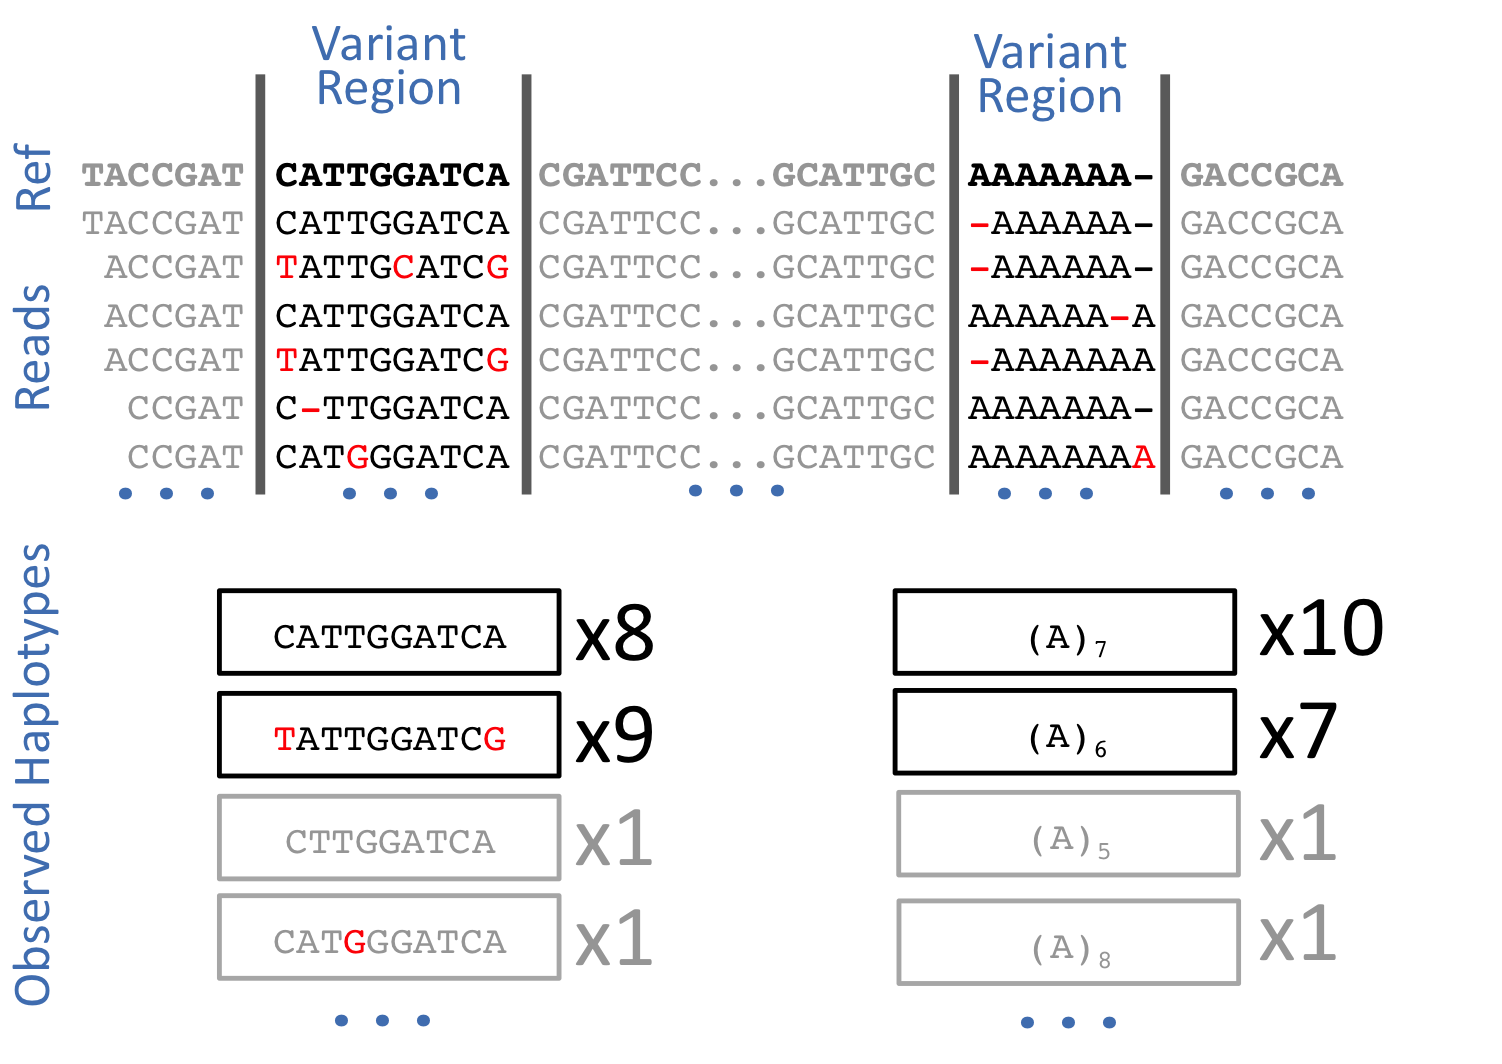
\includegraphics[width=0.8\textwidth]{haplotype_calling}
\caption{The direct detection of phase from short-read sequencing traces and counting of haplotypes across dynamically-determined windows.}
\label{fig:haplotypecalling}
\end{figure}

\subsection{Determining a window over which to assemble haplotype observations}

At each position in the reference, we collect allele observations derived from alignments as described in \ref{sec:parsing}.  To improve performance, we apply a set of input filters to exclude alleles from the analysis which are highly unlikely to be true.  These filters require a minimum number of alternate observations and a minimum sum of base qualities in a single sample in order to incorporate a putative allele and its observations into the analysis.

We then determine a haplotype length over which to genotype samples by a bounded iterative process.  We first determine the allele passing the input filters which is longest relative to the reference.  For instance, a longer allele could be a multi-base indel or a composite haplotype observation flanked by SNPs.  Then, we parse haplotype observations from all the alignments which fully overlap this window, finding the rightmost end of the longest haplotype allele which begins within the window.  This rightmost position is used to update the haplotype window length, and a new set of haplotype observations are assembled from the reads fully overlapping the new window.  This process repeats until the rightmost end of the window is not partially overlapped by any haplotype observations which pass the input filters. This method will converge given reads have finite length and the only reads which fully overlap the detection window are used in the analysis.

\subsection{Detection and genotyping of local haplotypes}
\label{sec:genotyping}

Once a window for analysis has been determined, we parse all fully-overlapping reads into haplotype observations which are anchored at the boundaries of the window.  Given these sets of sequencing observations $r_{i_1},\ldots,r_{i_{s_i}} = R_i$ and data likelihoods $P(R_i|G_i)$ for each sample and possible genotype derived from the putative alleles, we then determine the probability of polymorphism at the locus given the Bayesian model described in section \ref{sec:model}.

To establish a maximum \emph{a posteriori} estimate of the genotype for each sample, we employ a convergent gradient ascent approach to the posterior probability distribution over the mutual genotyping across all samples under our Bayesian model.  This process begins at the genotyping across all samples $G_1,\ldots,G_n$ where each sample's genotype is the maximum-likelihood genotype given the data likelihood $P(R_i|G_i)$:

\begin{equation}
G_1,\ldots,G_n =
\underset{G_i}{\operatorname{argmax}} \; P(R_i|G_i)
%:=  \{ G_i | \forall G : P(R_i|G_i) >= P(R_i|G) \}
\end{equation}

The posterior search then attempts to find a genotyping $G_1,\ldots,G_n$ in the local space of genotypings which has higher posterior probability under the model than this initial genotyping.  In practice, this step is done by searching through all genotypings in which a single sample has up to the $N$th best genotype when ranked by $P(R_i|G_i)$, and $N$ is a small number (e.g. 2).  This search starts with some set of genotypes $G_1,\ldots,G_n = \{G\}$ and attempts to find a genotyping $\{G\}'$ such that:

\begin{equation}
P(\{G\}'|R_1,\ldots,R_n) > P(\{G\}|R_1,\ldots,R_n)
\end{equation}

$\{G\}'$ is then used as a basis for the next update step.  This search iterates until convergence, but in practice must be bounded at a fixed number of steps in order to ensure optimal performance.  As the quality of input data increases in coverage and confidence, this search will converge more quickly because the maximum-likelihood estimate will lie closer to the maximum \emph{a posteriori} estimate under the model.

This method incorporates a basic form of genotype imputation into the detection method, which in practice improves the quality of raw genotypes produced in primary allele detection and genotyping relative to methods which only utilize a maximum-likelihood method to determine genotypes.  Furthermore, this method allows for the determination of marginal genotype likelihoods via the marginalization of assigned genotypes for each sample over the posterior probability distribution.

\subsection{Probability of polymorphism}

Provided a maximum \emph{a posteriori} estimate of the genotyping of all the individuals in our sample, we might like establish an estimate of the quality of the genotyping.  For this, we can use the probability that the locus is polymorphic, which means that the number of distinct alleles at the locus, $K$, is greater than 1.  While in practice the space of possible genotypings is too great to integrate over, it is possible to derive the probability that the loci is polymorphic in our samples by summing across the monomorphic cases:

\begin{equation}
\label{eq:probpoly}
P(K > 1 | R_1,\ldots,R_n)
=
1 - P(K = 1 | R_1,\ldots,R_n)
%=
%1 - \sum_{\forall(G_i,\ldots,G_n : K = 1)} P(G_i,\ldots,G_n|R_i,\ldots,R_n)
\end{equation}

Equation (\ref{eq:probpoly}) thus provides the probability of polymorphism at the site, which is provided as a quality estimate for each evaluated locus in the output of FreeBayes.

\subsection{Marginal likelihoods of individual genotypes}

Similarly, we can establish a quality estimate for a single genotype by summing over the marginal probability of that specific genotype and sample combination under the model.  The marginal probability of a given genotype is thus:

\begin{equation}
\label{eq:marginals}
P(G_j|R_i,\ldots,R_n)
=
\sum_{\forall(\{G\} : G_j \in \{G\})}
P(\{G\}|R_i,\ldots,R_n)
\end{equation}

In implementation, the estimation of this term requires us to must sample enough genotypings from the posterior in order to obtain well-normalized marginal likelihoods.  In practice, we marginalize from the local space of genotypings in which each individual genotype is no more than a small number of steps in one sample from the maximum \emph{a posteriori} estimate of $G_i,\ldots,G_n$.  This space is similar to that used during the posterior search described in section \ref{sec:genotyping}.  We apply (\ref{eq:marginals}) to it to estimate marginal genotype likelihoods for the most likely individual genotypes, which are provided for each sample at each site in the output of our implementation.

%\subsection{Extensions to the method}




%

%\subsection{Using prior empirical information to improve detection}

\bibliography{references}{}
%\bibliographystyle{plainnat}
\bibliographystyle{genome_research}

\end{document}
